\section{Results}\label{sec:results} 

In this section, we describe the results of our experiments.  We explore which
non-mainstream resolvers are available; how
the performance of mainstream resolvers compares to that of non-mainstream
resolvers; and whether (and to what extent) encrypted DNS response time
correlates to high network latency. We also explore how resolvers perform 
differently from home networks versus EC2 instances. 

\paragraph{Are Non-Mainstream Resolvers Available?}
We first aimed to study the availability of encrypted DNS
resolvers. 
We received responses from most resolvers that we queried. When trying to perform DoH queries from all vantage points,
we received 5,098,281 successful responses and 311,351 errors. 
The most common errors we received from attempting to communicate with
the resolvers were related to a failure to establish a connection or a segmentation fault.
We did not identify a consistent pattern of not receiving responses from a certain
subset of resolvers each time the measurements ran. 


\begin{figure}[h!]
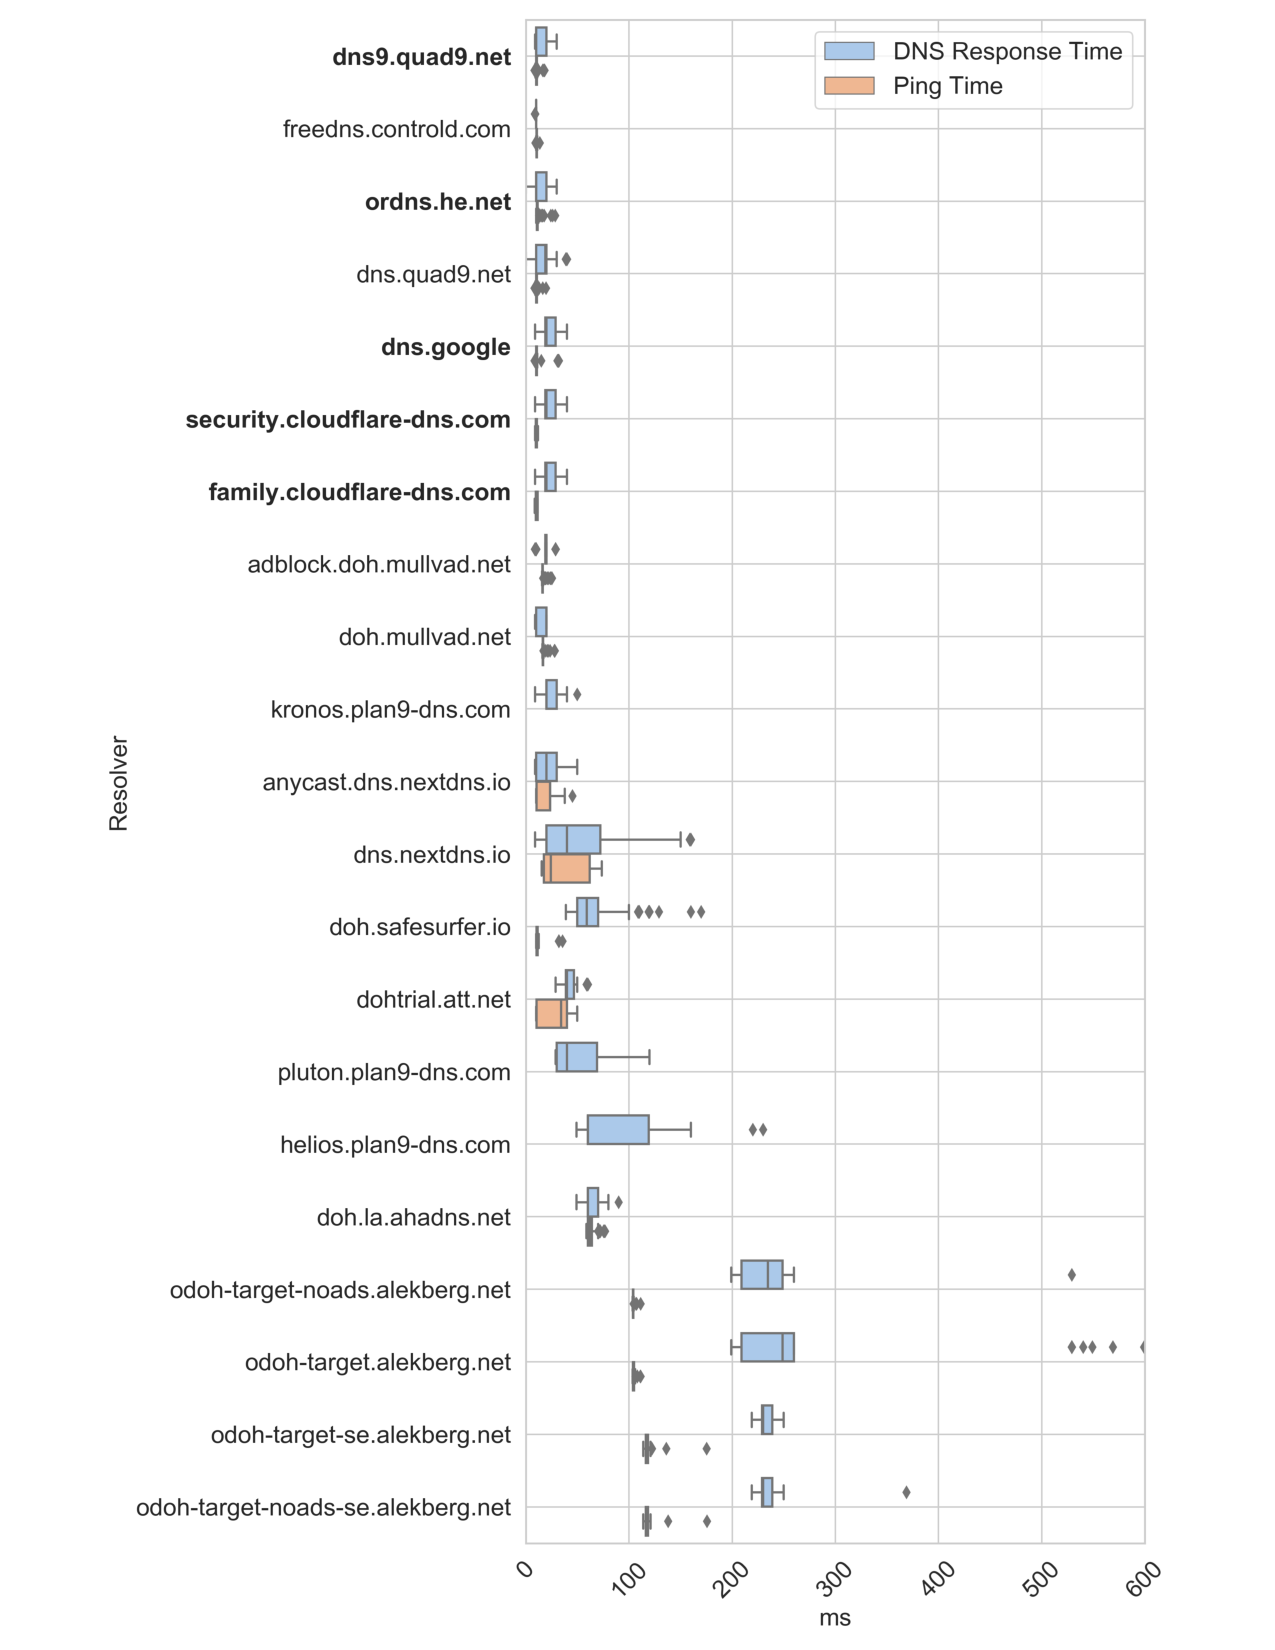
\includegraphics[width=\columnwidth]{ohio_NA}
\caption{The DNS response time and ICMP ping time distributions for
    encrypted DNS resolvers located in North America, measured from an EC2
    instance in Ohio.  The plots show distributions for both DNS response times
    and ICMP round-trip latency.}
    \label{fig:dns-us-ohio}
\end{figure}


\paragraph{How Do Non-Mainstream Resolvers Perform?}
Given the large number of non-mainstream resolvers that have not been
previously studied, we aimed to study how
the performance of these encrypted DNS resolvers compared to mainstream ones.
As previously mentioned, one of our motivations in doing so is to better
understand the global extent of encrypted DNS resolver deployment, as existing
lists of public encrypted DNS resolvers~\cite{dnscrypt-public-resolvers} do
not provide any overview of either reliability or performance. Additionally,
given that most organizations who have deployed mainstream resolvers are based
in the United States, we also wanted to explore how the performance of a
broader set of encrypted DNS resolvers varied by geography.

Figure~\ref{fig:dns-us-ohio} shows the distributions of DNS response times and
ICMP ping times across encrypted DNS resolvers located in North America, as
measured from an EC2 instance in Ohio.  The plots show distributions for both
DNS response times and ICMP round-trip latency.  Although some distributions
extend beyond 600~ms, we have truncated the plots for ease of exposition,
since responses beyond this range will not result in good application
performance.  Certain resolvers did not respond to our ICMP ping probes; for
those resolvers, no latency data is shown.
As expected, most mainstream resolvers outperformed non-mainstream resolvers
from most vantage points.  Non-mainstream resolvers also exhibited higher
variability of median query response times.  
From the Chicago home network devices, response times from resolvers were as
high as 399~ms, identified as much above typical DNS lookup response times.
From the Ohio vantage point, the maximum response time from a resolver was 270~ms. 

We also explored the distributions of DNS response times and ICMP ping times
across encrypted DNS resolvers located across continents, as measured from
vantage points in the United States, Asia, and Europe, respectively.  From
Seoul, the maximum response time from a resolver was 569~ms; from Frankfurt,
the maximum response time from a resolver was 380~ms.  We observe more
consistent performance for resolvers located in Europe, but we still note high
variability from the Seoul vantage point.
Figures~\ref{fig:dns-us}--\ref{fig:dns-europe} in the Appendix show all of
these results in more detail.

In some cases, one particular non-mainstream resolver would outperform
the mainstream DoH resolvers.  As expected, \texttt{dns.quad9.net},
\texttt{dns.google}, and \texttt{dns.cloudflare.com} were among the top five
highest performing DoH resolvers in North America, Europe, and Asia.
Interestingly, however, \texttt{ordns.he.net}---a DoH resolver hosted by
Hurricane Electric, a global Internet service provider (ISP)---managed to
outperform all mainstream resolvers from the home network devices. From Frankfurt, \texttt{dns.brahma.world}
outperforms \texttt{dns.cloudflare.com}; from Seoul, \texttt{dns.alidns.com} outperforms \texttt{dns.quad9.net},
\texttt{dns.google}, and \texttt{dns.cloudflare.com}; and from Ohio, \texttt{freedns.controld.com} outperforms \texttt{dns.google}
and \texttt{dns.cloudflare.com}.

We observe that the measurements performed from home network devices 
demonstrate fewer variability than the measurements performed from EC2 instances, 
especially the Seoul instance. Despite a few outliers, such as \texttt{doh.la.ahadns.net}, 
the graphs do not demonstrate high variabiility. Notably, the median resolver response 
times are almost identical for the home network and Ohio EC2 measurements. 


\begin{table}[t!]
\centering
\begin{tabular}{l|rr}
\toprule
    \textbf{Resolver} & \multicolumn{2}{c}{\textbf{Vantage Point}} \\
                  & \textrm{Seoul (ms)}         & \textrm{Frankfurt (ms)} \\
\midrule
antivirus.bebasid.com                                & 99 & 380                            \\
dns.twnic.tw                          & 59                                          & 290                              \\
dnslow.me                                & 29                                           & 240                              \\
jp.tiar.app                            & 39                                           & 250                             \\
public.dns.iij.jp                              & 39.5                                           & 250                               \\
\bottomrule
\end{tabular}
    \caption{Median DNS response times for non-mainstream resolvers (Asia).}
\label{tab:UnconvAsia}
\end{table}

\begin{table}[t!]
\centering
\begin{tabular}{l|rr}
\toprule
\textbf{Resolver} & \multicolumn{2}{c}{\textbf{Vantage Point}} \\
                  & \textrm{Frankfurt (ms)}     & \textrm{Seoul (ms)} \\
\midrule
doh.ffmuc.net                               & 70 & 569                         \\
dns0.eu                        & 20 & 399                         \\
open.dns0.eu         & 10 & 324                         \\
kids.dns0.eu                                 & 10 & 309                         \\
dns.njal.la                        & 20 & 289                         \\
\bottomrule
\end{tabular}
    \caption{Median DNS response times for non-mainstream resolvers (Europe).}
\label{tab:UnconvEur}
\end{table}


To better understand the extent to which certain encrypted DNS resolvers
perform well for clients in some regions but not others, we identified
resolvers that exhibited low DNS response times in for clients in one region
but not another. 
Tables~\ref{tab:UnconvAsia} and~\ref{tab:UnconvEur} show 
the five encrypted DNS resolvers for Europe and Asia that exhibit the 
largest differences in median DNS response times when
queried from a remote vantage point (queries of resolvers in Asia from Europe,
and of resolvers of Europe from Asia, respectively). In both cases, 
Table~\ref{tab:UnconvAsia} shows that non-mainstream resolvers located
in Asia perform better from the vantage point in Seoul than the one in
Frankfurt.  Similarly, as expected, Table~\ref{tab:UnconvEur} shows that the
median response times of non-mainstream resolvers in Europe are much lower when
measured from Frankfurt than the response times of those same resolvers
measured from Seoul.
